\documentclass{standalone}
\usepackage[dvipsnames]{xcolor}
\RequirePackage{tikz}
\usetikzlibrary{backgrounds}
\usetikzlibrary{hobby} 
\definecolor{thesisblue}{rgb}{.15, .15, .6}
\usepackage{pgfplots}
\pgfplotsset{compat=1.11}

\begin{document}

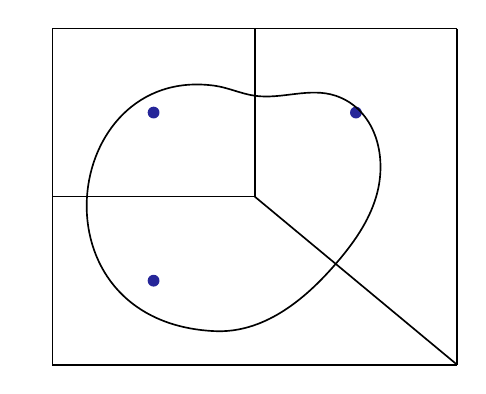
\begin{tikzpicture}[scale=1.5, use Hobby shortcut]
\begin{axis}[
  trig format plots=rad,
  hide axis,
  xmin=-0.5,
  xmax=1.5,
  ymin=-0.5,
  ymax=1.5]
  
    \draw (0, 0) -- (0, 1);
    \draw (0, 1) -- (1, 1);
    \draw (1, 1) -- (1, 0);
    \draw (1, 0) -- (0, 0);
    
    \fill[thesisblue] (0.25, 0.25) circle (0.05cm);
    \fill[thesisblue] (0.25, 0.75) circle (0.05cm);
    \fill[thesisblue] (0.75, 0.75) circle (0.05cm);

    %\path[draw,closed=true] (0.7,0.6) .. (0.4,0.1) .. (0.2, 0.8);
    
    \path[draw,closed=true] (0.7,0.3) .. (0.4,0.1) .. (0.4, 0.83) .. (0.5, 0.8) .. (0.7, 0.8) .. (0.8, 0.5);
    
    \draw[thin] (0,0.5) -- (0.5, 0.5);
    \draw[thin] (0.5, 0.5) -- (0.5, 1);
    \draw[thin] (0.5, 0.5) -- (1, 0); 

\end{axis}
\end{tikzpicture}
\end{document}
